\section{Qwen-RobotManip: The Generalizable Vision-Language-Action Model Design}
\label{sec:model}

\subsection{Main Architecture}

\ours follows a decoupled architecture consisting of a vision-language backbone for multimodal perception and semantic reasoning, and a flow-matching action expert for continuous action generation. This decoupling allows the action expert to specialize in high-frequency, fine-grained motor control while the backbone retains and extends its pretrained perceptual and reasoning capabilities through joint end-to-end training.

\paragraph{Vision-language backbone.}
We adopt Qwen3.5-4B~\citep{qwen35blog} as the vision-language backbone.
Qwen3.5 is a natively multimodal model trained with early vision-language fusion: visual tokens from a Vision Transformer with dynamic-resolution spatial merging are interleaved directly into the text token stream and processed uniformly across images and language instructions within a single transformer.
% Its hybrid attention design combines gated linear attention in the majority of layers with grouped-query softmax attention at regular intervals, allowing efficient encoding of long multimodal sequences while retaining full-precision global reasoning where needed.
Given one or more camera views together with a natural language task instruction, the backbone encodes them jointly into contextual representations (\eg, last-layer hidden states $D_{\mathrm{vlm}}{=}2560$) that capture both fine-grained visual features and task-level semantics, which are then consumed by the action expert via cross-attention.

\paragraph{Action expert.}
We attach a Diffusion Transformer (DiT)~\citep{peebles2023scalable} as a flow-matching action expert~\citep{chi2023diffusion,black2024pi0,adaptdiffuser} for learning precise continuous actions from both robot trajectory data and egocentric human demonstrations.
The expert consists of $N{=}10$ transformer blocks with hidden dimension $D_{\mathrm{act}}{=}768$ and 12 attention heads.
Each block performs self-attention over the concatenated state-and-action token sequence, followed by cross-attention to VLM hidden states and a SwiGLU feed-forward network.
Cross-attention layers alternate between attending to \emph{visual} tokens (even-indexed blocks) and \emph{language} tokens (odd-indexed blocks), both extracted from the final layer of the VLM, letting the expert separately ground action predictions in spatial observations and linguistic instructions at each processing stage.
The robot's proprioceptive state is encoded by a two-layer MLP and prepended to the noisy action token sequence before entering the DiT blocks. The expert is further conditioned on denoising timestep embeddings and additional learned camera embeddings detailed in \cref{subsec:cam_delta_action}.

% Besides, the robot's proprioceptive state is separately encoded by a two-layer MLP and prepended to the noisy action token sequence before entering the DiT blocks.
% The expert is conditioned on the denoising timestep embeddings, and additional learned camera embeddings detailed in \cref{subsec:cam_delta_action}.

The expert is trained with a flow-matching objective~\citep{lipman2023flow,esser2024scaling}. Given a ground-truth action chunk $\mathbf{a}$, a timestep $t \sim \mathrm{Beta}(1, 1.5)$ is sampled and an interpolant $\mathbf{x}_t = (1{-}t)\,\boldsymbol{\epsilon} + t\,\mathbf{a}$ is constructed from Gaussian noise $\boldsymbol{\epsilon}\sim\mathcal{N}(\mathbf{0},\mathbf{I})$. The model is then trained to minimize mean squared error on the predicted velocity field $\mathbf{x}_1 - \mathbf{x}_0$. At inference, action sequences are produced via 4 Euler integration steps, enabling low-latency real-time control. 
% This decoupled architecture lets the action expert specialize in high-frequency, fine-grained action generation while preserving the backbone's pretrained multimodal reasoning capabilities through joint training.

\begin{figure}[t]
    \centering
    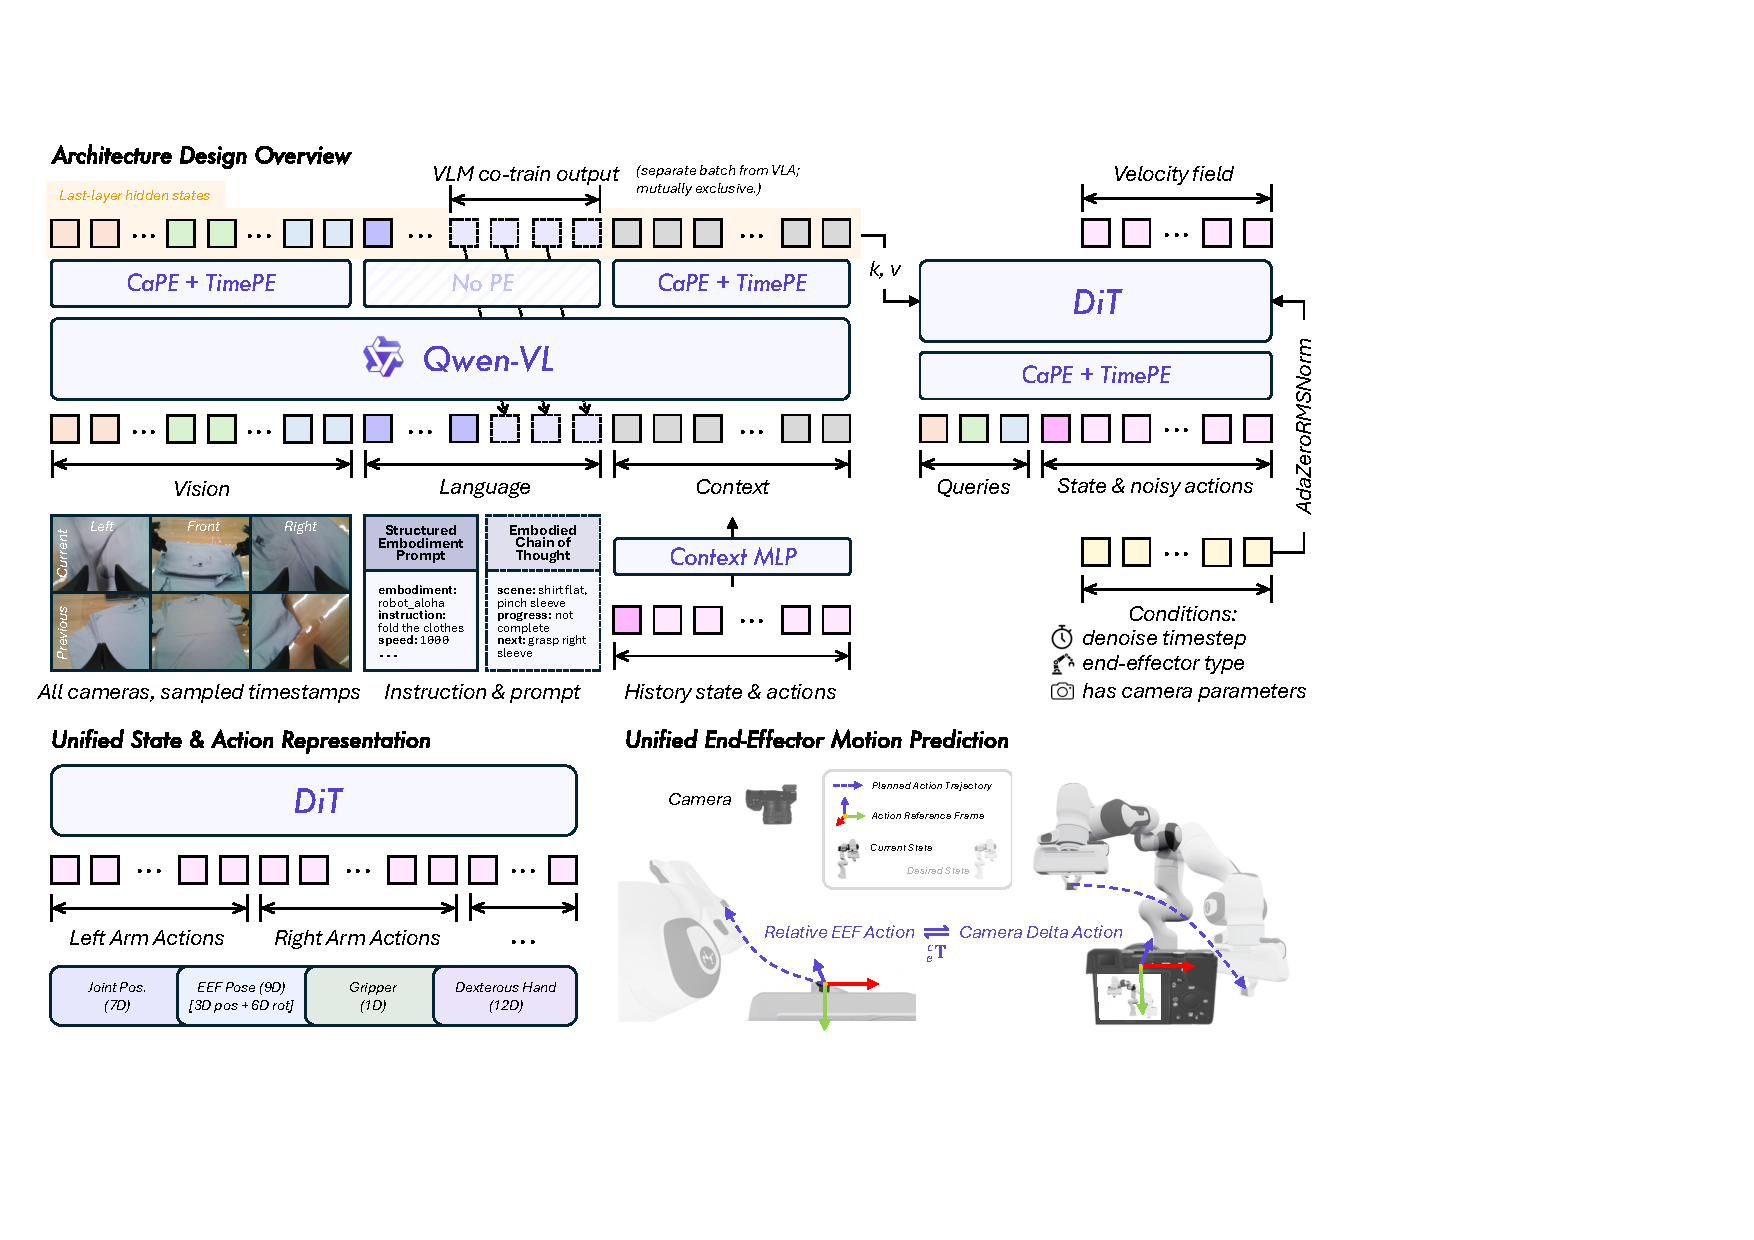
\includegraphics[width=0.99\linewidth]{figures/method-0616.pdf}
    \caption{\textbf{Overview of \ours.} The model couples a Qwen-VL backbone with a flow-matching Diffusion Transformer (DiT) action head. The backbone jointly encodes multi-view visual tokens, structured embodiment prompts, and historical context tokens, with last-layer hidden states injected into the DiT via alternating cross-attention. States and actions share a unified 80-dimensional canonical representation, with end-effector actions expressed as camera-frame delta poses to align the action space with visual observations across embodiments, conditioned on camera and end-effector type embeddings for embodiment-aware denoising. 
    VLM co-training and VLA training use separate batches, where each batch contains either (Vision, QA) or (Vision, Language, Context, Action) data.}
    \label{fig:method}
\end{figure}

\subsection{Cross-Embodiment State and Action Representation}
\label{sec:unified_state_action}

Heterogeneous proprioceptive states and action spaces across embodiments make scalable training on mixed multi-embodiment datasets a key challenge.
We address this by introducing an \textbf{80-dimensional canonical vector representation} for states and actions.  
The representation is structured as two 29-dimensional per-arm blocks followed by 22 reserved dimensions.
Each per-arm block is organized into the following semantic groups:
\begin{itemize}[leftmargin=*,topsep=2pt,itemsep=1pt]
    \item \textbf{Joint positions} (7 dims): joint positions for the robot arm;
    \item \textbf{End-effector pose} (9 dims): Cartesian position (3) and orientation in a 6D continuous rotation representation~\citep{zhou2019continuity} (6);
    \item \textbf{Gripper state} (1 dim): joint position for the parallel gripper;
    \item \textbf{Dexterous hand joints} (12 dims): active hand joint positions for embodiments equipped with multi-fingered dexterous hands.
\end{itemize}
The trailing 22 reserved dimensions are shared across both arms and are available for additional degrees of freedom such as mobile-base velocity.
For the \emph{state} vector, all values are expressed in absolute coordinates.
%For the \emph{action} vector, joint and end-effector values are expressed as relative deltas from the current state (\cref{subsec:cam_delta_action} details the specific end-effector delta representation).
For the \emph{action} vector, joint actions are expressed as absolute values and end-effector actions are expressed as relative deltas from the current state. In particular, end-effector orientation deltas are parameterized as 3D rotation vectors rather than the 6D representations used for states. \cref{subsec:cam_delta_action} further details the camera-frame delta representation for end-effector actions.


Different robot embodiments populate different subsets of this canonical template.
For example, a 7-DOF single-arm gripper (\eg, Franka Panda) fills the joint, end-effector, and gripper fields of one arm, leaving the remaining dimensions as zero.
A dual-arm system (\eg, ALOHA) fills both per-arm blocks. A robot with dexterous hands additionally populates the hand-joint dimensions. Zero-padded dimensions are excluded from the training loss via a per-dimension binary mask, ensuring that gradients flow only through semantically populated entries and preventing spurious supervision on structurally absent degrees of freedom.

\subsection{Unified End-Effector Motion Prediction}\label{subsec:cam_delta_action}

The canonical state-action representation of \cref{sec:unified_state_action} unifies the structural layout of states and actions across embodiments, but does not yet address a subtler source of fragmentation: end-effector poses recorded in different coordinate frames across datasets~\citep{lyu2026lda}. When the same motion is expressed relative to different base frames or camera frames depending on the data source, the model must learn to reconcile these geometric inconsistencies rather than focusing on the underlying manipulation skill. We address this by grounding all end-effector actions in a shared camera-frame delta pose representation and injecting camera geometry directly into the action expert via positional encodings. Together with embodiment-aware conditioning, this ensures that actions which appear visually similar are numerically proximate across embodiments, enabling the model to extract cross-embodiment synergies from heterogeneous data.

Concretely, we extract $N_{\mathrm{ee}} \in \{1, 2\}$ independent \textbf{40-dimensional per-end-effector tokens} from the 80-dimensional state-action vector. The 29 active dimensions of each arm are packed into a 40-dimensional slot with 11 reserved for future extension, and the DiT processes these tokens jointly via self-attention.

% To ground these per-end-effector action predictions in the visual domain, we pair this per-arm factorization with a \emph{camera-frame delta pose} action representation, \emph{camera-aware positional encodings}, and \emph{end-effector-aware conditioning} within the DiT.

\paragraph{Camera-frame delta pose action representation.}
Rather than representing end-effector motion as an absolute pose in the robot base frame, a relative pose in the end-effector local frame, or a world-frame delta, we adopt a \emph{camera-frame delta pose} representation~\citep{chen2025toward}. 
% The pose component of the unified action space can be represented in multiple ways: the absolute pose in the robot base frame, the relative pose in the end-effector's local frame, or a delta pose expressed in the world frame.
% We instead adopt a \emph{camera-frame delta pose} representation.
Its key property is that actions appearing visually similar in the image are also numerically proximate in the action space, directly aligning the action representation with the visual observation space and facilitating cross-embodiment transfer.
This requires calibrated camera intrinsics and extrinsics at both training and inference.

Formally, let $c$ denote the reference camera frame, $e$ the current end-effector frame, and $e^*$ the desired end-effector frame at a future step.
The pose component of the predicted action is:
\begin{equation}
\label{eqn:cam_delta_rot_inv}
    \mathbf{a}_p = \begin{bmatrix}
        \ ^c _e \mathbf{R} \ ^e_{e^*} \mathbf{R} \ ^e _c \mathbf{R} & \ ^c_e \mathbf{R} \ ^e \mathbf{t}_{e^*} \\
        \mathbf{0} & 1
    \end{bmatrix}
\end{equation}
The rotational block ${}^c_e\mathbf{R}\ {}^e_{e^*}\mathbf{R}\ {}^e_c\mathbf{R}$ expresses the relative end-effector rotation ${}^e_{e^*}\mathbf{R}$ in the camera frame by conjugating with the camera-to-end-effector extrinsics, while the translational block ${}^c_e\mathbf{R}\ {}^e\mathbf{t}_{e^*}$ projects the desired end-effector displacement into camera coordinates. The full expression is thus geometrically equivalent to projecting the relative end-effector action into the camera frame via the extrinsics.
A more compact alternative is~\citep{zhang2026grounding}:
\begin{equation}
\label{eqn: cam_delta_full_inv}
    \mathbf{a}_p = \ ^c _{e^*} \mathbf{T} \ ^e _c \mathbf{T}
\end{equation}
While \cref{eqn: cam_delta_full_inv} eliminates end-effector definition inconsistencies entirely, its translational component is coupled with the relative end-effector rotation ${}^e_{e^*}\mathbf{R}$ and the camera-to-end-effector offset ${}^e\mathbf{t}_c$, making it more susceptible to long-tail distributions and more sensitive to calibration errors.
We therefore adopt \cref{eqn:cam_delta_rot_inv} in implementation.

\paragraph{Camera-aware positional encoding.}
To enable the action expert to reason about camera geometry, we inject camera parameters into the DiT's cross-attention layers via Camera Positional Encoding (CaPE)~\citep{kong2024eschernet}.
Camera pose is encoded via CaPE, occupying 32 of each 64-dimensional attention head's dimensions, with the remaining 32 used by RoPE~\citep{heo2024rotary} for temporal indexing.
Each image token's positional encoding is derived from the extrinsics of its corresponding camera, while each state/action token uses the extrinsics of its selected reference camera.
Because CaPE is a rotational positional encoding, the global world-frame origin cancels algebraically in the dot-product attention, leaving only the relative pose between each visual token and the querying state/action tokens.

Following the practice of GTA~\citep{miyato2024gta} and PRoPE~\citep{li2025cameras}, we apply CaPE not only to keys and queries but also to values and attention outputs, strengthening the geometric consistency of the cross-attention.
Camera intrinsics are incorporated by projecting the normalized image-plane coordinates of each visual patch through a learned linear layer and adding them to the corresponding image token, providing per-token field-of-view awareness.

\paragraph{End-effector-aware conditioning.}

Beyond the denoising timestep, the DiT is further conditioned on two additional signals, both applied via additive embeddings through adaptive layer normalization~\citep{peebles2023scalable}.
\begin{enumerate}[leftmargin=*,topsep=2pt,itemsep=1pt]
    \item \emph{End-effector type embedding}: a learned codebook entry per end-effector category (single-arm, dual-arm left, dual-arm right, egocentric head, or mobile base) associated with each state/action token, allowing the model to apply embodiment-specific action priors.
    \item \emph{Auxiliary flag embedding}: a binary embedding indicating whether calibrated camera parameters are available for the current sample, switching the predicted pose action space between camera-frame delta mode and robot-base relative mode.
\end{enumerate}
% All three conditioning signals (timestep embedding, end-effector type, and auxiliary flag) are summed element-wise and fed to each DiT block through adaptive layer normalization~\citep{peebles2023scalable}.

\paragraph{Multi-view reference camera selection.}
In multi-view settings, the end-effector action is expressed relative to a chosen reference camera frame.
During training, for single-arm datasets we randomly select any available external or wrist-mounted view as the reference. For dual-arm datasets, we randomly apply one of two strategies:
(1) both arms share a head-mounted camera or any available third-person view as the common reference frame;
(2) the left arm uses the left wrist camera and the right arm uses the right wrist camera as their respective reference frames.

% TODO: add a figure illustrating the reference camera pose selection under the two strategies

Within the DiT's cross-attention, each image token uses the pose of its corresponding camera for CaPE, while each state/action token uses the pose of its selected reference camera for CaPE, guiding the DiT to denoise the camera delta action expressed in that reference frame.
Because CaPE is a rotational encoding, inter-view relative poses are encoded implicitly, with the world-frame superscript canceling algebraically.
%Notably, because CaPE is a rotational positional encoding, the world-frame superscript cancels algebraically in the attention, leaving only inter-view relative poses.
%The encoding thus simultaneously designates the reference viewpoint for each end-effector action and explicitly encodes the relative geometry among all available views.


\subsection{Embodiment Prompt}
% We adopt a structured prompt design composed of five components: embodiment, instruction, subtask, speed, and fps. The embodiment field specifies the robot platform (e.g., robot\_franka), enabling the model to account for differences in morphology and control characteristics across embodiments. The instruction field provides the high-level task specification (e.g., Pick an apple), defining the overall objective of the current episode. The subtask field optionally describes an intermediate step of the task, offering finer-grained guidance for sequential or long-horizon execution, although it may also be left empty when such information is unavailable. In addition, the speed field indicates the desired execution pace, and the fps field specifies the temporal sampling rate of the input sequence, both of which provide useful information about the dynamics of the demonstrated behavior.

% \begin{center}
% \begin{tikzpicture}
% \node[
%   draw=blue!40!black,
%   fill=blue!8,
%   rounded corners=3pt,
%   line width=0.7pt,
%   inner sep=4pt,
%   text width=0.70\linewidth,
%   align=left,
%   font=\ttfamily\footnotesize
% ] {
% embodiment: robot\_aloha\\
% instruction: Take the toy off the table and put it on the mat.\\
% speed: 1000\\
% fps: 30
% };
% \end{tikzpicture}
% \end{center}


% This prompt design allows the model to capture not only what task should be performed, but also important contextual factors related to which robot is acting and how the behavior is temporally executed. Such structured conditioning helps reduce ambiguity in policy learning, improves adaptability across different robot embodiments, and increases robustness to variations in trajectory speed and frame rate. To further improve flexibility, we randomly drop several prompt components, including embodiment, speed, and fps, with a probability of 15\% during training. This dropout strategy encourages the model to handle incomplete prompt information and improves generalization when some fields are unavailable at test time.

We adopt a structured prompt to condition the policy on both task semantics and execution context. 
Each prompt consists of the following fields:
\begin{itemize}[leftmargin=*,topsep=2pt,itemsep=1pt]
    \item \textbf{Embodiment}: the robot platform (\eg, \texttt{robot\_aloha}), enabling the model to account for morphological and control differences across embodiments.
    \item \textbf{Instruction}: the high-level task description, defining the overall objective of the episode.
    \item \textbf{Speed}: the episode length in timesteps, discretized into bins of 500 steps.
    \item \textbf{FPS}: the temporal sampling rate of the input sequence.
    \item \textbf{Camera View Direction}: the camera's position relative to the robot arm, either \texttt{arm side} or \texttt{opposite side}.
    
\end{itemize}
% Each prompt consists of the following components:
% \begin{itemize}
%     \item \textbf{Embodiment}: the robot platform used in the current episode (e.g., \texttt{robot\_aloha}), allowing the model to adapt to differences in morphology and control characteristics across embodiments.
    
%     \item \textbf{Instruction}: the high-level task specification (e.g., \textit{Take the toy off the table and put it on the mat}), defining the overall objective of the episode.
    
%     \item \textbf{Speed}: the episode length in timesteps, discretized into bins of 500 steps.

    
%     \item \textbf{FPS}: the frame rate of the input sequence, indicating the temporal resolution of the demonstration.
% \end{itemize}


% An example prompt is shown below:
% \vspace{0.3em}

\begin{center}
\begin{tcolorbox}[
  width=0.72\linewidth,
  colback=gray!6!white,
  colframe=gray!50!black,
  colbacktitle=gray!40!black,
  coltitle=white,
  title={\small\bfseries Structured Embodiment Prompt Example},
  arc=5pt,
  boxrule=0.8pt,
  titlerule=0pt,
  left=8pt, right=8pt, top=6pt, bottom=6pt,
]
{\color{gray!60!black}\textbf{embodiment:}}~{\color{gray!60!black}\texttt{robot\_aloha}}\\[2pt]
{\color{gray!60!black}\textbf{instruction:}}~{\color{gray!60!black}\texttt{Take the toy off the table and put it on the mat.}}\\[2pt]
{\color{gray!60!black}\textbf{speed:}}~{\color{gray!60!black}\texttt{1000}}\\[2pt]
{\color{gray!60!black}\textbf{fps:}}~{\color{gray!60!black}\texttt{30}} \\[2pt]
{\color{gray!60!black}\textbf{camera view direction:}}~{\color{gray!60!black}\texttt{arm side}}
\end{tcolorbox}
\end{center}

Together, these fields allow the model to capture not only what task should be performed, but also which robot is acting and how the behavior is temporally structured, 
reducing ambiguity in policy learning, improving adaptability across embodiments, and increasing robustness to variations in execution speed and frame rate. 
To further improve robustness to incomplete inputs, we randomly drop the embodiment, speed, and fps fields with probability 15\% during training, encouraging the model to generalize when prompt information is partially unavailable at test time.



%% Draft: In-Context Policy Adaptation Section
%% For: StarVLA / VLA paper
%% Language: English

%% Draft: In-Context Policy Adaptation Section
%% For: StarVLA / VLA paper
%% Language: English

%% Draft: In-Context Policy Adaptation Section
%% For: StarVLA / VLA paper
%% Language: English

\subsection{In-Context Policy Adaptation}
\label{sec:in_context}

Despite the strong generalization enabled by cross-embodiment pretraining, deploying a VLA policy to a new robot or environment often requires rapid behavioral adaptation without parameter updates. Inspired by in-context learning in large language models, we equip \ours{} with an in-context policy adaptation mechanism that conditions current action prediction on a structured window of recent execution history (observation-action pairs) from the same episode, enabling the policy to adapt its behavior at deployment time without any parameter update or task-specific fine-tuning.

\paragraph{Execution context representation.}
A key design question is what information constitutes a useful policy context. We draw a direct analogy from the model's own inference procedure. At each decision step, \ours{} observes the current visual observations and proprioceptive state and predicts a complete action chunk of $K$ steps. We therefore define one context chunk as exactly this triplet $(\mathbf{o}_h, \mathbf{s}_h, \mathbf{a}_h)$, consisting of the visual observation, proprioceptive state, and the $K$-step action sequence executed during chunk $h$. This records what the robot saw, was in, and did. A context of $H$ such chunks thus provides the policy with a structured window of recent behavior it can directly reason about.

The two modalities within each context chunk are processed through complementary pathways, owing to their fundamentally different representational structures. Historical frames $\mathbf{o}_h$ are prepended to the current frame and processed jointly by the VLM visual encoder within a single forward pass, with an image-count annotation appended to the language instruction to help the VLM attribute each visual token to its correct temporal position. Proprioceptive states and action chunks, which cannot be processed by the visual pathway, are projected into the VLM hidden space by two lightweight MLP encoders. The state encoder $\mathrm{MLP}_s$ and action encoder $\mathrm{MLP}_a$ produce per-chunk token representations with learned temporal position embeddings $\mathbf{e}_h^{\mathrm{temp}}$ to distinguish chunks and slot embeddings $\mathbf{e}_{0:K'}^{\mathrm{slot}}$ to distinguish action tokens within each chunk:
\begin{align}
    \mathbf{t}_h^s
        &= \mathrm{MLP}_s(\mathbf{s}_h)
           + \mathbf{e}_h^{\mathrm{temp}}
        \;\in\; \mathbb{R}^{D_\mathrm{vlm}},
    \label{eq:state_tok}\\
    \bigl[\mathbf{t}_h^{a,0},\ldots,\mathbf{t}_h^{a,K'-1}\bigr]
        &= \mathrm{reshape}\!\left(
             \mathrm{MLP}_a\!\left(\mathrm{flatten}(\mathbf{a}_h)\right)
           \right)
           + \mathbf{e}_h^{\mathrm{temp}}
           + \mathbf{e}_{0:K'}^{\mathrm{slot}}
        \;\in\; \mathbb{R}^{K' \times D_\mathrm{vlm}}.
    \label{eq:action_tok}
\end{align}
All $H$ chunks are serialized chronologically into a single context token sequence:
\begin{equation}
    \mathbf{C} = \bigl[
        \underbrace{\mathbf{t}_0^s,\;\mathbf{t}_0^{a,0{:}K'}}_{\text{chunk }0},\;
        \underbrace{\mathbf{t}_1^s,\;\mathbf{t}_1^{a,0{:}K'}}_{\text{chunk }1},\;
        \ldots,\;
        \underbrace{\mathbf{t}_{H-1}^s,\;\mathbf{t}_{H-1}^{a,0{:}K'}}_{\text{chunk }H-1}
    \bigr]
    \;\in\; \mathbb{R}^{H(1+K') \times D_\mathrm{vlm}}.
    \label{eq:ctx_seq}
\end{equation}
The current state $\mathbf{s}_t$ is not encoded here and continues to flow through the action head's dedicated state encoder unchanged, preserving full backward compatibility with the base \ours{} model.

\paragraph{History integration.}
We study two strategies for injecting context token sequence into the policy. In the \emph{unified} mode, context tokens $\mathbf{C}$ are appended to the end of the VLM input sequence and processed jointly with visual and language tokens under causal self-attention, allowing the VLM to reason over history, task description, and visual observations together. The resulting history-fused last-layer hidden states are passed to the DiT action head via cross-attention. In the \emph{dual} mode, the state-action context is injected directly into the DiT action head rather than the VLM, keeping the VLM context length unchanged at the cost of shallower history integration. Unified injection allows the VLM's full self-attention to jointly reason over behavioral history, task description, and visual observations, enabling richer cross-modal context integration than is possible when history is confined to the action head alone. We therefore adopt unified injection as the default configuration.

\paragraph{Stochastic context sampling.}
A naive strategy of always providing the $H$ most recent chunks leads to a degenerate shortcut. Because the last context chunk is temporally closest to the current step, the model can achieve low training loss by simply copying the most recent action chunk rather than genuinely reasoning about the episode's behavioral dynamics. This collapses the context mechanism into a trivial action-copy heuristic, which breaks down whenever the immediate history is ambiguous, atypical, or does not reflect the robot's broader execution style. What we want the model to learn is the behavioral profile of the current episode~\citep{huang2025dadu}, its velocity patterns, grasping strategies, and interaction signatures, not a shortcut based on temporal proximity. 
To prevent this, we introduce \textit{stochastic context sampling} during training. Rather than always supplying the $H$ chunks immediately preceding the current step, the context window is drawn from a random position within the episode. The sampled chunks may therefore be temporally distant from the current step, forcing the model to reason about the robot's behavioral profile across the full episode rather than exploiting recency as a shortcut. 

This randomization serves as a form of curriculum diversification. The model must learn to extract consistent behavioral style from \emph{any} subset of the episode history, making it robust to missing, partial, or temporally displaced context at inference time. 
At deployment, we supply a rolling window of the most recent $H$ chunks as context, allowing the model to leverage the full available history.
Empirically, stochastic context sampling proves critical for preventing this collapse. Without it, the policy achieves low training loss but poor task success, a clear sign that the model has learned to copy recent actions rather than reason about execution context. With it, the model genuinely exhibits in-context adaptation, adjusting its behavior based on the broader behavioral dynamics of the current episode.
